\subsection{Espelhamento Vertical}

\begin{listing}[H]
    \caption{Comando \texttt{esp.vertical}}

    \begin{minted}{python}
        def espelhamento_vertical(imagem):
            return imagem[::-1]
    \end{minted}
\end{listing}

Pode ser implementado também com \pyline{cv2.flip(imagem, 0)} \autocite{ref:flip}.

\begin{figure}[H]
    \centering
    \begin{subfigure}{0.45\textwidth}
        \centering
        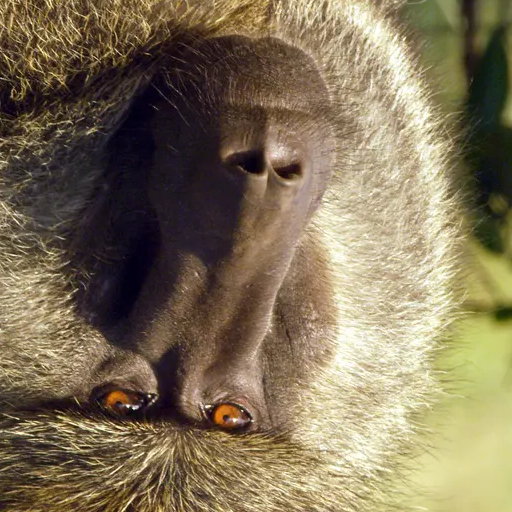
\includegraphics[width=6cm]{resultados/colorflip.png}
        \caption{\texttt{imagens/color.png}}
    \end{subfigure}%
    \begin{subfigure}{0.45\textwidth}
        \centering
        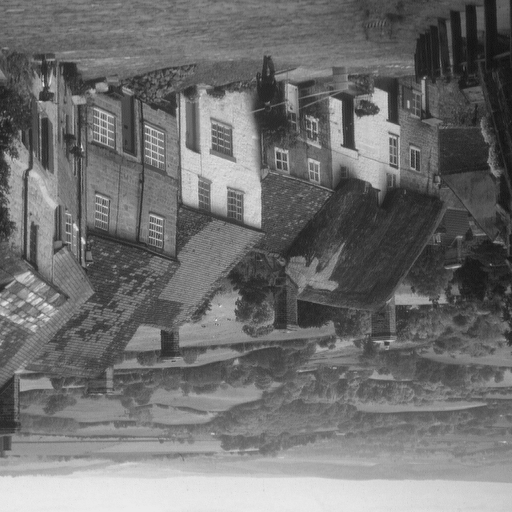
\includegraphics[width=6cm]{resultados/cityflip.png}
        \caption{\texttt{imagens/city.png}}
    \end{subfigure}

    \caption{Imagem espelhada verticalmente.}
\end{figure}
